\documentclass[a4paper,12pt]{article} % добавить leqno в [] для нумерации слева
\usepackage[a4paper,top=1.3cm,bottom=2cm,left=1.5cm,right=1.5cm,marginparwidth=0.75cm]{geometry}
%%% Работа с русским языком
\usepackage{cmap}					% поиск в PDF
\usepackage{mathtext} 				% русские буквы в фомулах
\usepackage[T2A]{fontenc}			% кодировка
\usepackage[utf8]{inputenc}			% кодировка исходного текста
\usepackage[english,russian]{babel}	% локализация и переносы
\usepackage{siunitx}

\usepackage{graphicx}

\usepackage{wrapfig}
\usepackage{tabularx}

\usepackage{hyperref}
\usepackage[rgb]{xcolor}
\hypersetup{
colorlinks=true,urlcolor=blue
}

%%% Дополнительная работа с математикой
\usepackage{amsmath,amsfonts,amssymb,amsthm,mathtools} % AMS
\usepackage{icomma} % "Умная" запятая: $0,2$ --- число, $0, 2$ --- перечисление

%% Номера формул
\mathtoolsset{showonlyrefs=true} % Показывать номера только у тех формул, на которые есть \eqref{} в тексте.

%% Шрифты
\usepackage{euscript}	 % Шрифт Евклид
\usepackage{mathrsfs} % Красивый матшрифт

%% Свои команды
\DeclareMathOperator{\sgn}{\mathop{sgn}}

%% Перенос знаков в формулах (по Львовскому)
\newcommand*{\hm}[1]{#1\nobreak\discretionary{}
{\hbox{$\mathsurround=0pt #1$}}{}}

%%% Заголовок
\author{Макаров Лев Евгеньевич}
\title{Лабораторная работа №1.1.1

Определение систематических и случайных погрешностей при измерении удельного сопротивления нихромовой проволоки
}
\date{\today}

\begin{document}

\begin{titlepage}
	\begin{center}
		{\large МОСКОВСКИЙ ФИЗИКО-ТЕХНИЧЕСКИЙ ИНСТИТУТ (НАЦИОНАЛЬНЫЙ ИССЛЕДОВАТЕЛЬСКИЙ УНИВЕРСИТЕТ)}
	\end{center}
	\begin{center}
		{\large Физтех-школа фотоники, электроники и молекулярной физики}
	\end{center}
	
	
	\vspace{4.5cm}
	{\huge
		\begin{center}
			{\bf Отчёт о выполнении лабораторной работы 1.1.1}\\
			Определение систематических и случайных погрешностей при измерении удельного сопротивления нихромовой проволоки
		\end{center}
	}
	\vspace{2cm}
	\begin{flushright}
		{\LARGE Автор:\\ Макаров Лев Евгеньевич \\
			\vspace{0.2cm}
			Б04-306}
	\end{flushright}
	\vspace{8cm}
	\begin{center}
		Долгопрудный 2023
	\end{center}
\end{titlepage}

\section{Введение}

\textbf{Цель работы:} измерить удельное сопротивление проволоки и вычислить систематические и случайные погрешности при использовании таких измерительных приборов, как линейка, штангенциркуль, микрометр, амперметр, вольтметр и мост постоянного тока.
\medskip

\textbf{В работе используются:} 
\begin{itemize}
    \item линейка
    \item штангенциркуль
    \item микрометр
    \item отрезок проволоки из нихрома
    \item амперметр
    \item вольтметр
    \item источник ЭДС
    \item мост постоянного тока
    \item реостат
    \item ключ
\end{itemize}
\medskip

В работе используются следующие методы измерения сопротивления:
\begin{enumerate}
	\item определение углового коэффициента наклона зависимости напряжения на проволоке от тока через неё;
	\item измерение с помощью моста постоянного тока.
\end{enumerate}

\section{Теоретические сведения}

Удельное сопротивления однородной проволоки круглого сечения можно определить по следующей формуле:

\begin{equation}\label{1form}
\rho = R \frac{S}{l},
\end{equation}

\noindent где $R$ -- сопротивление проволоки, $S$ -- её площадь, $l$ -- длина.

\begin{equation}\label{1form}
S = \frac{\pi d^2}{4},
\end{equation}

\noindent где $d$ -- диаметр проволоки.

\medskip

\begin{wrapfigure}{r}{4cm}
	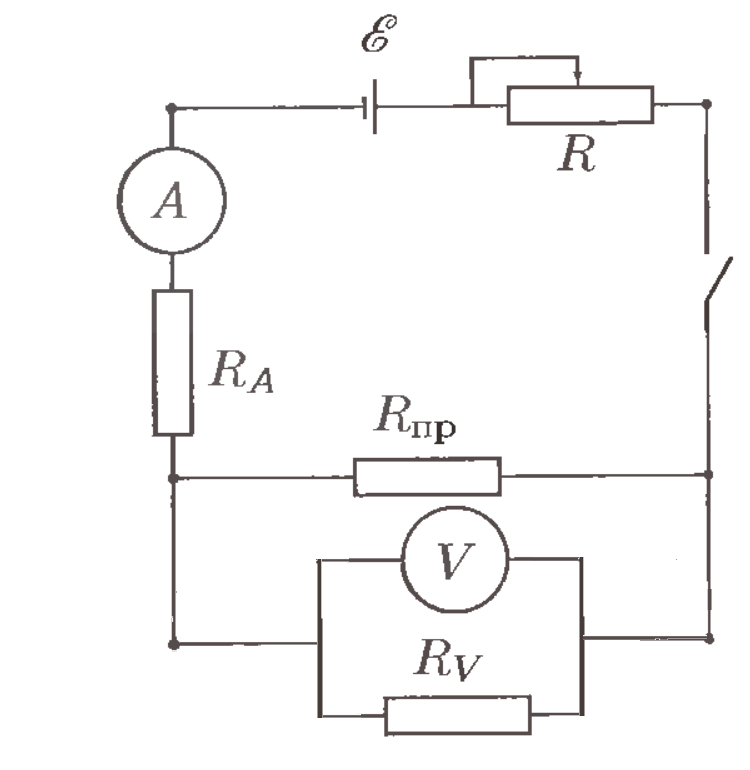
\includegraphics[width=4cm]{scheme.png}
	\caption{\textit{Схема цепи}}
	\label{fig:image}
\end{wrapfigure}

Согласно закону Ома напряжение $V$ и ток $I$ в образце связаны соотношением

\begin{equation}
V = RI.
\end{equation}

Для измерения напряжения и тока используем схему на \textit{рис.  \ref{fig:image}}.

\medskip

Т.к. используемый вольтметр неидеален необходимо сделать поправку на его сопротивление $R_V$.

\medskip

Показания амперметра $I_A$ и вольтметра $V_\text{В}$ связаны следующим соотношением

\begin{equation}
V_\text{В}=R^\prime I_A,
\end{equation}

\noindent где $R^\prime$ -- сопротивление параллельно соединённых проволоки и~вольтметра.

\medskip

При этом $\frac{1}{R^\prime} = \frac{1}{R_V} + \frac{1}{R}$, и $R_V \gg R, R^\prime$.\\

Таким образом, график зависимости $V_\text{В}\left(I_A\right)$ должен представлять прямую, угловой коэффициент которой есть $R^\prime$, откуда сопротивление образца может быть найдено по следующей формуле:

\begin{equation}\label{r_provoloki}
R = \dfrac{R_V R^\prime}{R_V - R^\prime} \approx R^\prime \left( 1 + \frac{R^\prime}{R_V} \right) 
\end{equation}

\section{Оборудование и экспериментальные погрешности}

\textbf{Штангенциркуль:} $\Delta_\text{шт} = \pm 0,1$ мм \\
\textbf{Микрометр:} $\Delta_\text{мкм} = \pm 0,01 $ мм \\
\textbf{Основные характеристики приборов:} 

\begin{tabular}[]{|l|l|l|}
\hline
Характеристика & Вольтметр & Амперметр \\
\hline
Система & Магнито-электрическая & Цифровая \\
\hline
Класс точности & 0,5 & — \\
\hline
Предел измерений $x_n$ & 0,75 В & 2 А \\
\hline
Число делений шкалы $n$ & 150 & — \\
\hline
Цена деления $x_n/n$ & $5 \cdot 10^{-3} \text{ В}$ & — \\
\hline
Чувствительность $n/x_n$ & 200 дел./В & — \\
\hline
Абсолютная погрешность $\Delta x_M$ & $\pm3,75\text{ мВ}$ & $\pm(0,002x + 0,02)\text{ мА}$ \\
\hline
Внутреннее сопротивление& 5000 Ом & 1,4 Ом \\
\hline
\end{tabular}\\

\medskip

Известно, что $R$ по порядку величины $\approx 5 \text{ Ом}$. Так как $R_V = 5000 \text{ Ом}$, то погрешность измерений для схемы составляет $\approx 0,001 = 0,1 \%$. Поэтому она пренебрежимо мала и не оказывает значительног овлияния на последующие измерения, а значит далее будем считать, что:

\begin{equation}
R\approx R^\prime
\end{equation}\\

\noindent\textbf{Мост постоянного тока P4833:}\\
\begin{tabular}{|p{8cm}|p{7cm}|}
	\hline
	Класс точности&0,1 \\
	\hline
	Разрядность магазина сопротивлений& 5 ед. \\
	\hline
	Исследуемый диапазон измерений& $ 10^{-4} - 10 \text{ Ом} $ (для множителя $ N = 10^{-2} $) \\
	\hline
	Погрешность измерений в используемом диапазоне& $\pm0,01\text{ Ом}$ \\
	\hline
\end{tabular}\\

\section{Результаты измерений и обработка данных}

\subsection{Измерение диаметра $d$ проволоки}

Измерения проводились штангенциркулем и микрометром для $N = 10$ различных участков проволоки. При измерении получено:

\begin{table}[h]
\begin{tabular}{|l|l|l|l|l|l|l|l|l|l|l|}
    \hline
    Номер   измерения & 1    & 2    & 3    & 4    & 5    & 6    & 7    & 8    & 9    & 10   \\ 
    \hline
    d, мм (штангенциркуль) & 0,4 & 0,4 & 0,4 & 0,4 & 0,4 & 0,4 & 0,4 & 0,4 & 0,4 & 0,4 \\ 
    \hline
    d, мм (микрометр) & 0,36 & 0,37 & 0,37 & 0,37 & 0,36 & 0,36 & 0,37 & 0,36 & 0,36 & 0,37 \\ 
    \hline
\end{tabular}\caption{\textit{Измерение диаметра проволоки микрометром и штангенциркулем}}
\end{table}

Среднее значение диаметра $ \overline{d} = \frac{\sum d_i}{N} = 0,365 \text{ мм}$.\\

Случайная погрешность измерения $ \sigma_{\overline{d}} = \sqrt{\frac{1}{N  (N-1)}\sum(d_i-\overline{d})^2} \approx 0,002 \text{ мм}$.\\

С учётом инструментальной погрешности $ \Delta_\text{мкм} = 0,01$ мм погрешность диаметра может быть вычислена как $ \sigma^{\text{полн}}_{\overline{d}} = \sqrt{\sigma^2_{\overline{d}} + \Delta^2_{\text{мкм}}} \approx 0,01 \text{ мм}$. \\

\textit{Окончательные результаты измерения диаметра проволоки:}

\begin{itemize}
	\item Штангенциркулем: $ d = 0,4 \pm 0,1 \text{ мм}  $
	\item Микрометром:  $ d = 0,365 \pm 0,010 \text{ мм} \left(\varepsilon = 2,8 \%\right)  $
\end{itemize}

Как видно, измерение микрометром гораздо точнее, чем измерение штангенциркулем, поэтому далее будем использовать его.
Вычислим площадь поперечного сечения проволоки $S$ из полученного диаметра:

\begin{equation}
S = \frac{\pi d^2}{4} = \frac{3,14 \cdot 0,365^2}{4} \approx 0,105 \text{ мм}^2
\end{equation}\\

Величину погрешности $\sigma_S$ найдём по формуле:

\begin{equation}
\sigma_S = 2\frac{\sigma^{\text{полн}}_{\overline{d}}}{d}S = 2 \cdot \frac{0,01}{0,365} \cdot 0,105  \approx 0,006 \text{ мм}^2
\end{equation}\\

Итак, $S = (0,105 \pm 0,006) \text{ мм}^2$, т.е площадь поперечного сечения определена с точностью $6 \%$.

\subsection{Измерение сопротивления проволоки}

Результаты измерений зависимостей показания вольтметра $ V_\text{В} $ от показаний амперметра $ I_A $ в схеме на \textit{рис.  \ref{fig:image}} представлены в \textit{Таблице \ref{tab:VotI}}. Соответствующие графики зависимостей изображены на \textit{рис. \ref{graph}}.\\

Пользуясь методом наименьших квадратов, строим аппроксимирующие прямые $ V_\text{В} = \overline{R}I_A $, определяя их угловой коэффициент по формуле

\begin{equation}
\overline{R} = \frac{\langle VI \rangle}{\langle I^2 \rangle}.
\end{equation}

\begin{figure}[h!]
	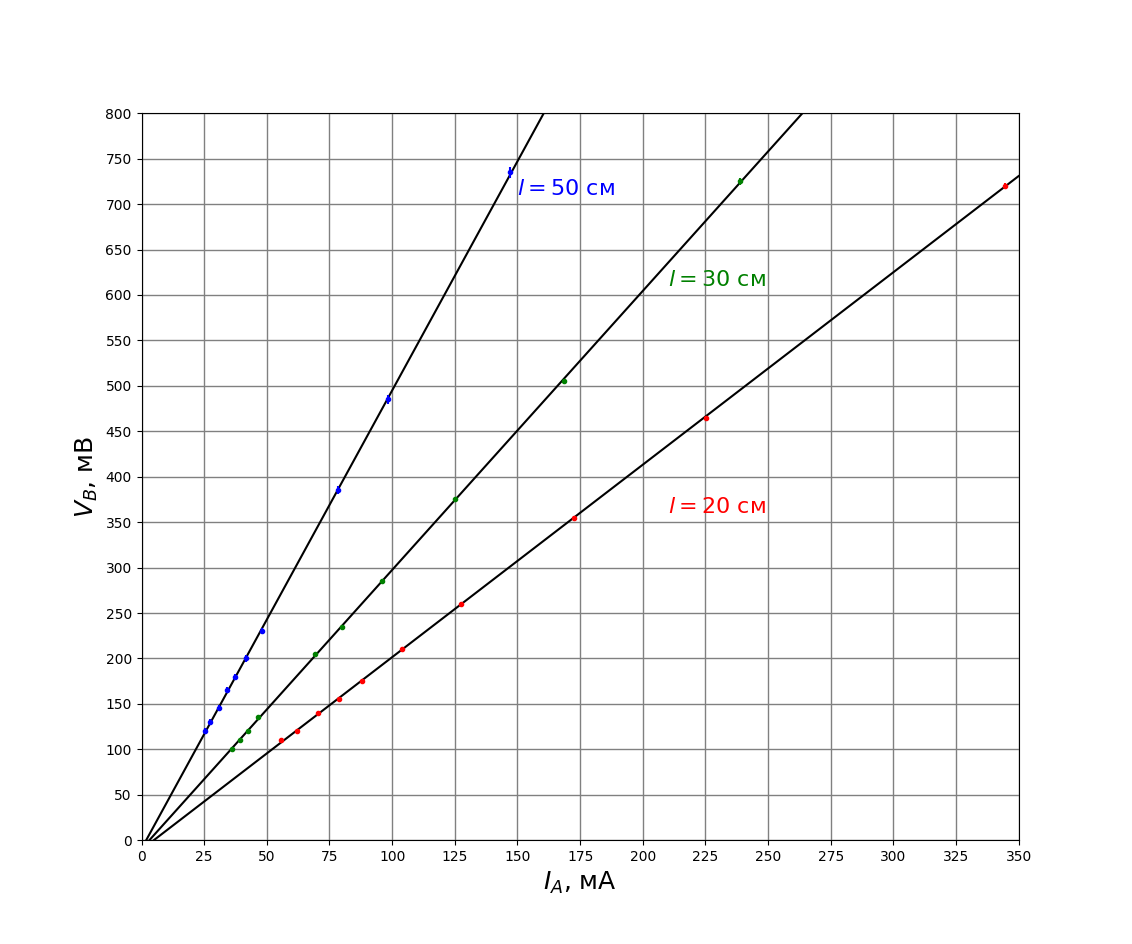
\includegraphics[width=1\linewidth]{graph.png}
	\caption{\textit{Результаты измерений напряжения $ V $ в зависимости от тока $ I $ для проволок разной длины $ l $ и их линейная аппроксимация $ y=kx $.}}
	\label{graph}
\end{figure}

\begin{table}[h!]
\begin{tabular}{|lll|lll|lll|}
\hline
\multicolumn{3}{|c|}{L = 20 см}                                                        & \multicolumn{3}{c|}{L =   30 см}                                                      & \multicolumn{3}{c|}{L =   50 см}                                                      \\ \hline
\multicolumn{1}{|c|}{V, дел} & \multicolumn{1}{c|}{V, мВ} & \multicolumn{1}{c|}{I, мА} & \multicolumn{1}{c|}{V, дел} & \multicolumn{1}{c|}{V, мВ} & \multicolumn{1}{c|}{I, мА} & \multicolumn{1}{c|}{V, дел} & \multicolumn{1}{c|}{V, мВ} & \multicolumn{1}{c|}{I, мА} \\ \hline
\multicolumn{1}{|l|}{144}    & \multicolumn{1}{l|}{720}   & 344,33                     & \multicolumn{1}{l|}{145}    & \multicolumn{1}{l|}{725}   & 238,86                     & \multicolumn{1}{l|}{147}    & \multicolumn{1}{l|}{735}   & 147,15                     \\ \hline
\multicolumn{1}{|l|}{93}     & \multicolumn{1}{l|}{465}   & 225,1                      & \multicolumn{1}{l|}{101}    & \multicolumn{1}{l|}{505}   & 168,5                      & \multicolumn{1}{l|}{97}     & \multicolumn{1}{l|}{485}   & 98,4                       \\ \hline
\multicolumn{1}{|l|}{71}     & \multicolumn{1}{l|}{355}   & 172,45                     & \multicolumn{1}{l|}{75}     & \multicolumn{1}{l|}{375}   & 125,04                     & \multicolumn{1}{l|}{77}     & \multicolumn{1}{l|}{385}   & 78,56                      \\ \hline
\multicolumn{1}{|l|}{52}     & \multicolumn{1}{l|}{260}   & 127,55                     & \multicolumn{1}{l|}{57}     & \multicolumn{1}{l|}{285}   & 95,78                      & \multicolumn{1}{l|}{46}     & \multicolumn{1}{l|}{230}   & 47,91                      \\ \hline
\multicolumn{1}{|l|}{42}     & \multicolumn{1}{l|}{210}   & 104,11                     & \multicolumn{1}{l|}{47}     & \multicolumn{1}{l|}{235}   & 79,84                      & \multicolumn{1}{l|}{40}     & \multicolumn{1}{l|}{200}   & 41,52                      \\ \hline
\multicolumn{1}{|l|}{35}     & \multicolumn{1}{l|}{175}   & 88,08                      & \multicolumn{1}{l|}{41}     & \multicolumn{1}{l|}{205}   & 69,39                      & \multicolumn{1}{l|}{36}     & \multicolumn{1}{l|}{180}   & 37,36                      \\ \hline
\multicolumn{1}{|l|}{31}     & \multicolumn{1}{l|}{155}   & 78,72                      & \multicolumn{1}{l|}{27}     & \multicolumn{1}{l|}{135}   & 46,6                       & \multicolumn{1}{l|}{33}     & \multicolumn{1}{l|}{165}   & 34,08                      \\ \hline
\multicolumn{1}{|l|}{28}     & \multicolumn{1}{l|}{140}   & 70,33                      & \multicolumn{1}{l|}{24}     & \multicolumn{1}{l|}{120}   & 42,41                      & \multicolumn{1}{l|}{29}     & \multicolumn{1}{l|}{145}   & 31,09                      \\ \hline
\multicolumn{1}{|l|}{24}     & \multicolumn{1}{l|}{120}   & 62,07                      & \multicolumn{1}{l|}{22}     & \multicolumn{1}{l|}{110}   & 39,23                      & \multicolumn{1}{l|}{26}     & \multicolumn{1}{l|}{130}   & 27,39                      \\ \hline
\multicolumn{1}{|l|}{22}     & \multicolumn{1}{l|}{110}   & 55,72                      & \multicolumn{1}{l|}{20}     & \multicolumn{1}{l|}{100}   & 36,02                      & \multicolumn{1}{l|}{24}     & \multicolumn{1}{l|}{120}   & 25,38                      \\ \hline
\end{tabular}
\caption{\textit{Зависимость $ V $ от $ I $ для разных длин проволоки $ l $.}}\label{tab:VotI}
\end{table}

Случайную погрешность определения углового коэффициента вычисляем как

\begin{equation}
\sigma^\text{сл}_R = \sqrt{\frac{1}{n-1}\left( \frac{\langle V^2\rangle}{\langle I^2 \rangle} - \overline{R}^2 \right) },
\end{equation}

где $ n = 10 $ -- число измерений.

Теперь оценим систематическую погрешность, которая возникает из-за неточности используемых приборов. Полагая, что при всех измерениях относительная погрешность неизменна, оценим погрешность вычисления частного $ R = V / I $ при максимальных значения $ V $ и $ I $:

\begin{equation}
\Delta^\text{сист}_R \approx R\sqrt{\left( \frac{\Delta_V}{V_{max}} \right)^2 + \left( \frac{\Delta_I}{I_{max}} \right)^2  }
\end{equation}

Тогда полная погрешность измерения $ R $ вычисляется следующим образом:

\begin{equation}
\sigma^\text{полн}_R = \sqrt{\left( \sigma^\text{сл}_R \right)^2 + \left( \Delta_R^\text{сист} \right)^2 }.
\end{equation}




\label{chetire}

Результаты вычислений приведены в \textit{Таблице \ref{tab:rezult}}. Там же представлены результаты измерения сопротивления при помощи моста P4833.

\begin{table}[h!]
	\begin{tabular}{|l|l|l|l|l|l|l|}
		\hline
		$l$, см & $\overline{R}$, Ом & $ \sigma_R^\text{сл} $, Ом & $ \sigma_R^\text{сист} $, Ом & $ \sigma_r^\text{полн} $, Ом & $ \varepsilon, \% $ & $ R_\text{мост} $, Ом \\ \hline
		20 & 2,063 & 0,012 & 0,012 & 0,017 & 0,85 & $ (2,125 \pm 0,010) $ \\ \hline
		30 & 3,000 & 0,016 & 0,018 & 0,024 & 0,81 & $ (3,133 \pm 0,010) $ \\ \hline
		50 & 4,929 & 0,027 & 0,030 & 0,040 & 0,81 & $ (5,140 \pm 0,010) $ \\ \hline
	\end{tabular}
\caption{\textit{Результаты измерения сопротивления проволоки}}
\label{tab:rezult}
\end{table}



	
	
Таким образом, относительная погрешность измерения сопротивления достаточно мала и находится на уровне $ 0,8\% $. Также вычисленные значения сопротивления достаточно хорошо совпадают с измерениями при помощи моста.	

\subsection{Вычисление удельного сопротивления}

По формуле \eqref{1form} находим удельное сопротивление материала проволоки, используя значения, полученные в п. \ref{chetire}. Относительную погрешность вычисления $ \rho $ определяем по следующей формуле и заносим результаты в \textit{таблицу \ref{rezi}}:


\begin{table}[h!]

	\begin{tabular}{|l|l|l|l|}
		\hline
		& $ \rho , \text{Ом} \cdot \text{мм}^2 / \text{м} $   & $ \sigma_p, \text{Ом} \cdot \text{мм}^2 / \text{м} $ & $ \varepsilon_\rho, \% $   \\ \hline
		$l$ = 20 см & 1,080 & 0,061 & 5,6 \\ \hline
		$l$ = 30 см & 1,046 & 0,059 & 5,6 \\ \hline
		$l$ = 50 см & 1,031 & 0,058 & 5,6 \\ \hline
	\end{tabular}
	\caption{\textit{Результат измерения удельного сопротивления}}\label{rezi}
\end{table}

\begin{equation}
\sigma_\rho = \rho \sqrt{\left( \frac{\sigma_R}{R}  \right)^2 + \left( \frac{\sigma_S}{S} \right) ^2 + \left( \frac{\sigma_l}{l} \right) ^2 }.
\end{equation}



Усредняя результаты трёх опытов, окончательно получаем:

\begin{equation}
\overline{\rho} = \left( 1,052 \pm 0,059 \right) \text{Ом} \cdot \text{мм}^2 / \text{м} \left( \varepsilon_\rho = 5,6 \% \right) 
\end{equation}

\section{Обсуждение результатов и выводы}

В ходы работы было получено значение удельного сопротивления нихромовой проволоки с точностью $ \sim 6 \% $. Поэтому при измерении сопротивления проволоки достаточна точность $ 3-4 \% $. \\
Табличное значение удельного сопротивления для нихрома при $ \SI{20}{\degreeCelsius} $ значения варьируются от $ 0,970 \text{ Ом} \cdot \text{мм}^2 / \text{м} $ до $ 1,120 \text{ Ом} \cdot \text{мм}^2 / \text{м} $ в зависимости от состава различных сплавов (согласно справочнику "Физические величины. М.: Энергоиздат, 1991. С. 444"). Измерения попадают в нужный диапазон, однако не позволяют определить конкретную марку сплава.

\medskip

\noindent 
Точность измерения удельного сопротивления $ \rho $ существенно ограничивается измерением
диаметра проволоки. Поскольку случайная ошибка измерения диаметра оказалась меньше
цены деления прибора (микрометра), уточнение значения диаметра за счет многократных измерений невозможно. По той же причине не удалось проверить, насколько однородной является проволока по сечению.
	
	
	
	
	
	
\end{document}